\documentclass{article}
\usepackage[utf8]{inputenc}
\usepackage[american]{babel}
\usepackage{csquotes}
\usepackage{hyperref}
\usepackage[backend=biber,style=numeric,hyperref=true,natbib=true,autocite=plain,sorting=none]{biblatex}

% gantt chart
\usepackage{pgfgantt}
\usepackage{rotating}
\usepackage[graphicx]{realboxes}

\newganttchartelement*{mymilestone}{
mymilestone/.style={
shape=isosceles triangle,
inner sep=0pt,
draw=cyan,
top color=white,
bottom color=cyan!50
},
mymilestone incomplete/.style={
/pgfgantt/mymilestone,
draw=yellow,
bottom color=yellow!50
},
mymilestone label font=\slshape,
mymilestone left shift=0pt,
mymilestone right shift=0pt
}

\newgantttimeslotformat{stardate}{%
\def\decomposestardate##1.##2\relax{%
\def\stardateyear{##1}\def\stardateday{##2}%
}%
\decomposestardate#1\relax%
\pgfcalendardatetojulian{\stardateyear-01-01}{#2}%
\advance#2 by-1\relax%
\advance#2 by\stardateday\relax%
}

% fix margins
\usepackage[margin=1in]{geometry}
%\usepackage{fixltx2e}

% add double space
\usepackage{setspace}
\doublespacing

% get csv data

\usepackage{csvsimple}

% this package and the below text is to force images to be added to the given section and subsection. See https://tex.stackexchange.com/questions/279/how-do-i-ensure-that-figures-appear-in-the-section-theyre-associated-with/235312#235312 for more information
\usepackage{placeins}
\let\Oldsection\section
\renewcommand{\section}{\FloatBarrier\Oldsection}

\let\Oldsubsection\subsection
\renewcommand{\subsection}{\FloatBarrier\Oldsubsection}

\let\Oldsubsubsection\subsubsection
\renewcommand{\subsubsection}{\FloatBarrier\Oldsubsubsection}

\addbibresource{references.bib}

\title{%
  Design III Report: Bridge Structure \\
	\large Stevens Institute of Technology}

\date{October 2018}
\author{Joshua Schmidt, Andrew Chesterman, Jordan Balgahoom}

\usepackage{graphicx}

\begin{document}

\maketitle

\bigskip
\bigskip
\bigskip
\bigskip

\begin{figure}[!htb]
  \centering
  \includegraphics[width=0.75\textwidth]{assets/before-busting-side.jpg}
  \label{fig:logo}
\end{figure}

\newpage

\tableofcontents

\newpage

% References to all attachments in the main body of the report

\section{Abstract}

The goal of this project was to create a two-dimensional structure that can has the highest support-force to material-length ratio. The minimum load that the structure needed to support was 325 lbf, with a maximum copper tubing material length of 70 cm. The final load to length ratio was 6.8, with a maximum supported load of 475 lbf and a length of 66.2 inches. The mass to length ratio of the final product was 1.36. Therefore, this project was successful in meeting and surpassing the original specified requirements.

\bigskip
\bigskip
\bigskip
\bigskip
\bigskip
\bigskip
\bigskip
\bigskip

\begin{figure}[!htb]
  \centering
  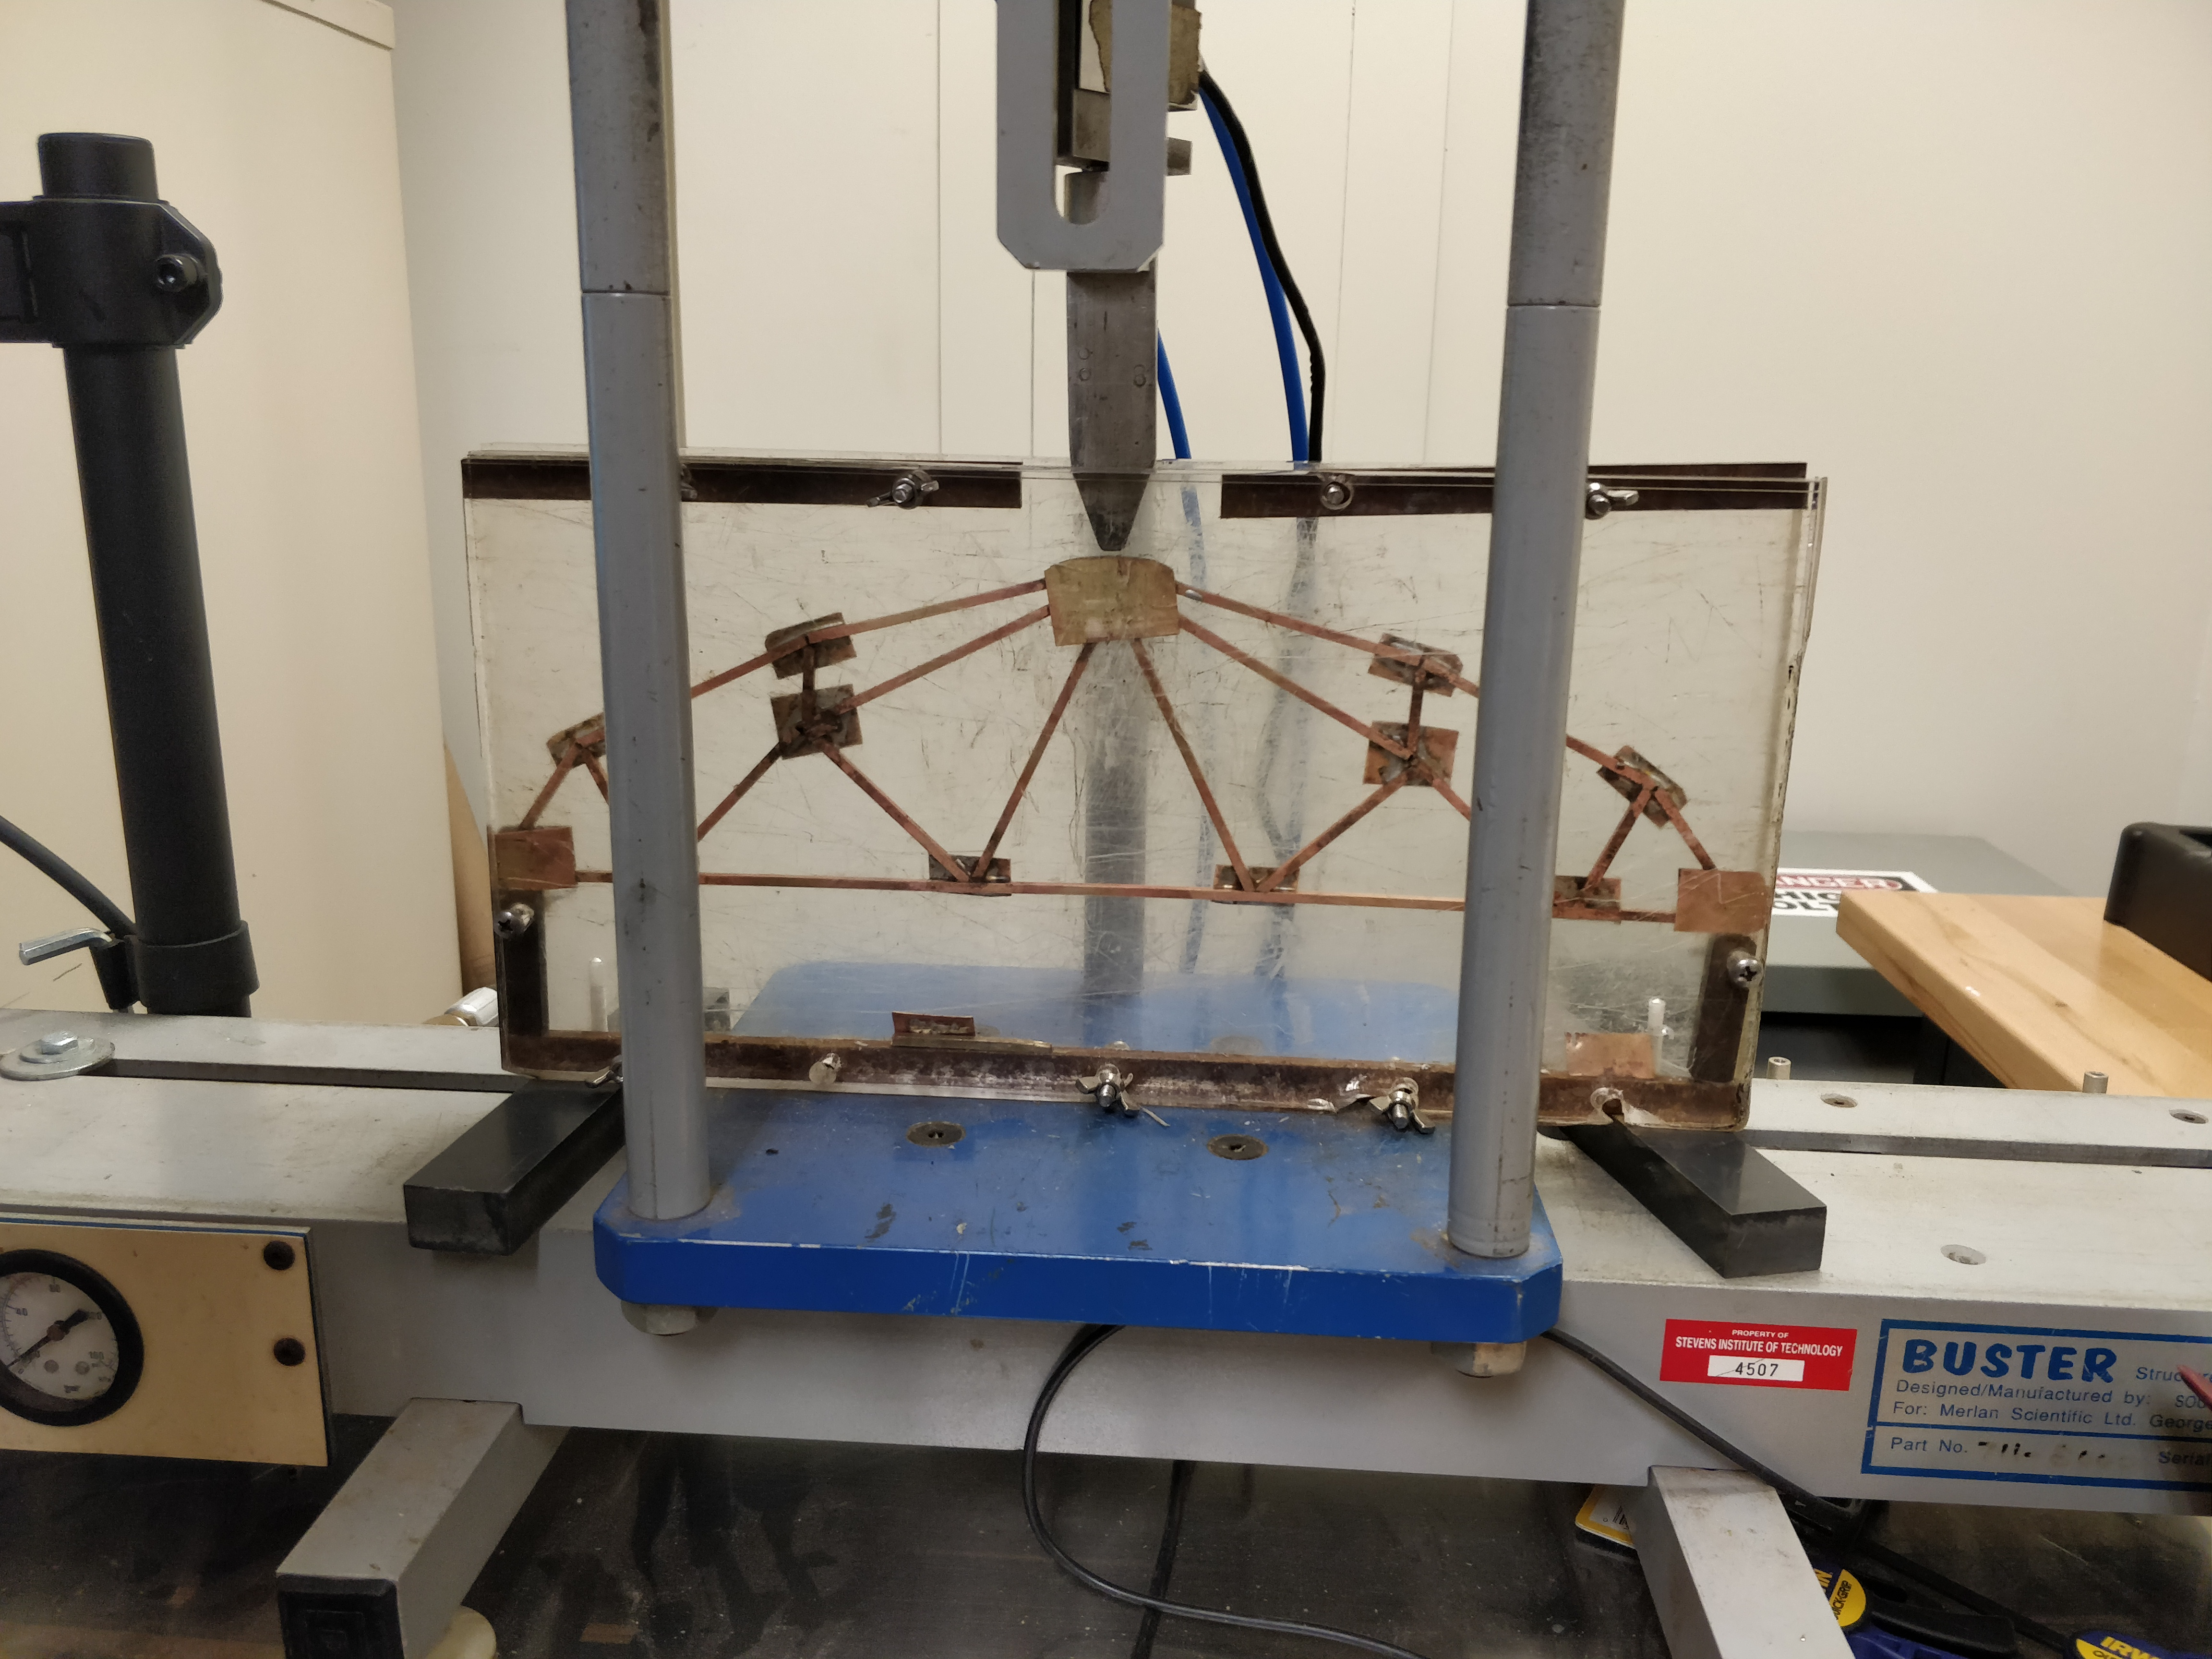
\includegraphics[width=0.75\textwidth]{assets/in-buster-close.jpg}
  \label{fig:truss-buster}
  \caption{Truss Buster}
\end{figure}

\newpage

\section{Introduction}

\subsection{Project objectives}

The main objective of this project was to design a planar truss that could support a given load over a given distance. Each team member had to design their own individual truss design before designing one final truss that would be used for testing. The final truss design was chosen because of its high load to failure, low amount of required material, and high strength to weight ratio. After all of these considerations, the truss was assembled by the team using the tools and materials provided to them.  


\subsection{Project Specifications}

\subsubsection{Requirements}

The truss had to support a minimum of 325 lb, and a maximum of 500 lb. It had to be no more than 4" in height, and had to span a 15" gap. It could not exceed 2" below the horizontal span. In addition, the truss had to rest flat on two 1/2" wide supports in the truss buster. The joints at the supports, and the joint where the load would be applied, all had to be double gusseted. The joint that would bear the load also had to be at the top of the truss. The truss had to be no thicker than 0.175" at any given point, otherwise it would not fit in the truss buster. 

\subsubsection{Materials}
\begin{itemize}
\item Full Scale Paper Template
\item (2)x 36" Long, 1/8" Square Brass Tubing
\item (1)x 12" Long, 0.016" x 1" Brass Strip
\item Butane Torch
\item Flux Paste
\item Flux Brush
\item Refractory Bricks
\item Fume Extractor
\item Bandsaw/Hacksaw
\item Sander/Sandpaper
\item Lead-Free Solder
\item Heat Resistant Mat
\item Safety Goggles
\item Gloves
\item Hand Shear
\end{itemize}

\subsection{Approach}

The team stuck to the general schedule that was provided to the class. Design and construction took two class periods each. Testing was done on the last day of construction as well. To complete this project in a timely fashion, we started by first coming up with the best design. This design needed to meet the requirements listed above, while additionally having the highest load to material use ratio. Once the design was selected, it was further refined in the truss analyzer until the highest ratio was attained. We then sketched the truss on a 1:1 scale, and started fabricating the truss out of copper. The goal was to finish the design in the first week, and complete fabrication within the next two weeks, with testing and analysis on the last week. These goals and the schedule were all met.

\newpage

\section{Discussion}

The design of the truss was the most important part of this project, as it determined how easily the truss would be fabricated and how much load could be handled. With this in mind, the team very carefully chose the design that was both relatively easy to fabricate and had the highest load to material use ratio, fulfilling the requirements listed prior.

\subsection{Design}

\subsubsection{Overview}

The team began designing their truss by experimenting in the Truss Analyzer application on the VLE. After some introduction to trusses in class, they played around with different designs to figure out what worked and what did not. They went through a few different designs, and after much discussion and collaboration, they decided on their final design. This design was the easiest to fabricate due to the fact it had more room for error with the use of less material and had the highest load to material use ratio, additionally fulfilling the extra credit design goal.

\begin{figure}[!htb]
  \centering
  \includegraphics[width=0.75\textwidth]{assets/maincuts.jpg}
  \label{fig:main-cuts}
  \caption{Initial Member Cuts}
\end{figure}

\subsubsection{Choice and Reasoning}

Each member of the team created their own trusses in the Truss Analyzer program on the VLE. The truss that was chosen out of the three individual truss designs was chosen due to its ability to hold more weight and use less material than the other two designs. While there was some concern due to the six member joint, the team chose this design anyway due to the effectiveness and efficiency of the design. This design also met the strength to length ratio for a full bonus two points on the design. The alternative designs held less weight than the chosen design and while they were simpler to build, they used more material than the chosen design, leaving less room for error. 

\subsubsection{Design Analysis summary}

The design chosen was predicted to hold 447 pounds. It was predicted to have buckled at four different members, being members one, three, seven, and eleven. Instead, the truss created was able to withstand 475 pounds and only buckled at member five. This may have been due to the fact that the team did not account for the thickness of the members when creating the truss on paper. This created the need to sand many inches off certain members so they would fit the truss that was designed, so that possibly added strength to certain members of the truss that should have failed at a lower amount of force. As for why only member five buckled under the force of the truss buster and not its symmetrical counterpart along with it, there could be a number of factors. One may be that the member itself was exposed to more heat than the other ones, making it weaker than the rest. It could have been more exposed to heat as the team started on that side of the truss the team was less experienced with soldering at the start before figuring out ways of soldering more effectively and efficiently.

\subsubsection{Fabrication}

One fabrication concern was the six member joint at the top of the truss. The more members that meet at a joint, the harder it is to solder. The team considered the difficulty of soldering this joint, and decided that, with enough practice, including the six member joint would greatly increase the strength of the truss. Another concern was if the four member joints were strong enough to hold their own without a double gusset. Thus, a fabrication consideration was to put double gussets on the four member joints to increase their strength. The team decided against this because there was concern that using less gusset for each joint just to strengthen these two joints could actually make the truss itself weaker than what was wanted and so the team stuck with only double gussets at the two end joints and the top joint. 

\begin{figure}[!htb]
  \centering
  \includegraphics[width=0.75\textwidth]{assets/before-busting-side-2.jpg}
  \label{fig:finished-truss}
  \caption{Finished Truss}
\end{figure}

\newpage

\section{Conclusion and Recommendations}

\subsection{Accomplishments}

The max load of the truss was 475 lb, which not only met, but exceeded the objective of the project. This max load was also far higher, 6.3\%, than the projected max load calculated by the truss analyzer. 66.2" of brass tubing was used, which was well under the maximum of 72". The truss also had a weight of 90g, which was fourth best in the class. Considering the mass to length ratio of the truss, which was 1.36, it was the second lowest in the class. In addition, the team was able to successfully solder the initially very daunting six member joint, which did not break at all during testing. The method of cutting at joints for many of the members was also a success because it allowed for easier construction and a stronger truss. This was used to turn the six member joint into a four member joint by cutting at the top member and the middle members and bending them.

\begin{figure}[!htb]
  \centering
  \includegraphics[width=0.75\textwidth]{assets/truss-busted-side.jpg}
  \label{fig:truss-busted-side}
  \caption{Truss Busted Side}
\end{figure}

\subsection{Recommendations}

Given the opportunity to redo the project, the team would do a few things differently. First of all, measurements would be more accurate. Initially, when drawing the design of paper, the width of the brass tubes was not accounted for, so the truss construction went a little bit differently than expected. Another likely change would be more soldering practice. With more practice, the joints would have been slightly stronger, especially at the double gusset joints. Also, less solder would be used, which would decrease the weight and increase the strength to weight ratio of the truss. One final recommendation would be to make sure that the height of the truss actually is no more than four inches, as when the team initially tested, the truss buster dented the top gusset joint, raising some concern, however the truss was able to withstand 475 pounds afterwards, so there was no big issue, but there could have been one.

\begin{figure}[!htb]
  \centering
  \includegraphics[width=0.75\textwidth]{assets/truss-busted-top.jpg}
  \label{fig:truss-busted-top}
  \caption{Truss Busted Top}
\end{figure}

\newpage

\begin{sidewaysfigure}

\section{Attachments}

\subsection{Work Chart / Gantt Chart}

\begin{ganttchart}[vgrid, hgrid]{1}{30}
\gantttitle{November}{30}\\
\gantttitlelist{1,...,30}{1}\\
%First Group
\ganttgroup{Design}{1}{7} \\
\ganttbar{Create Candidate Truss Designs}{1}{3} \\
\ganttbar{Analyze Designs Quantitatively}{4}{5} \\
\ganttbar{Choose Best Design}{6}{7}\\
\ganttmilestone{Completed Design Phase}{6}
\ganttnewline
\ganttlink{elem1}{elem2}
\ganttlink{elem2}{elem3}
%Second Group
\ganttgroup{Fabrication}{8}{20} \\
\ganttbar{Create Copper Tube Members}{8}{11} \\
\ganttbar{Sand Members and Create Gusset Plates}{12}{15} \\
\ganttbar{Solder Members and Gusset Plates Together}{16}{20}\\
\ganttmilestone{Completed Truss}{20}
\ganttlink{elem3}{elem4}
\ganttlink{elem4}{elem6}
\ganttlink{elem6}{elem7}
\ganttlink{elem7}{elem8}
\ganttnewline
%Third Group
\ganttgroup{Analysis}{21}{30} \\
\ganttbar{Truss Buster Analysis}{21}{22} \\
\ganttbar{Data Analysis}{23}{24} \\
\ganttbar{Report Writing}{25}{30}\\
\ganttmilestone{Completed Analysis}{30}
\ganttlink{elem8}{elem9}
\ganttlink{elem9}{elem11}
\ganttlink{elem11}{elem12}
\ganttlink{elem12}{elem13}
\ganttlink{elem13}{elem14}
\end{ganttchart}
\end{sidewaysfigure}

\newpage

\subsection{Truss Analysis}

\subsubsection{Forces}

\begin{figure}[!htb]
  \centering
  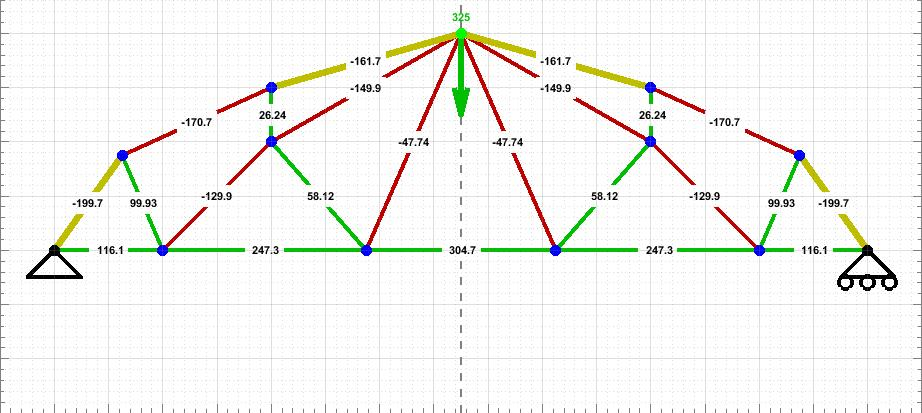
\includegraphics[width=0.75\textwidth]{assets/final_truss_1_forces.jpg}
  \label{fig:truss-forces-main}
  \caption{Final Design Forces}
\end{figure}

\subsubsection{Lengths}

\begin{figure}[!htb]
  \centering
  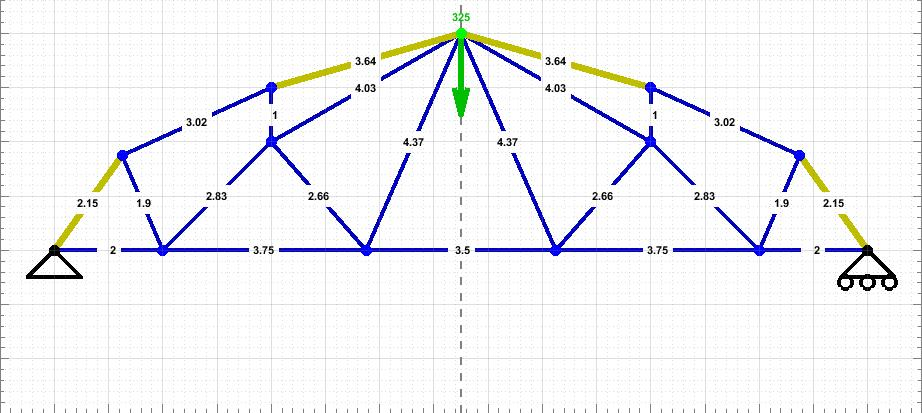
\includegraphics[width=0.75\textwidth]{assets/final_truss_1_lengths.jpg}
  \label{fig:truss-lengths-main}
  \caption{Final Design Lengths}
\end{figure}

\subsubsection{Data}

\centering
\csvautotabular{assets/final_truss_1.csv}

\newpage

\subsection{Alternatives Truss Analysis}

\subsubsection{Alternative 1}

Forces

\begin{figure}[!htb]
  \centering
  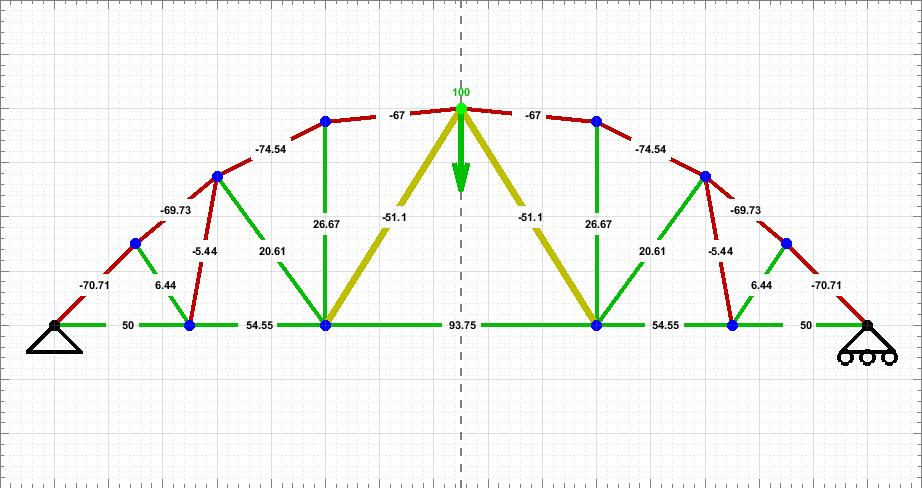
\includegraphics[width=0.75\textwidth]{assets/final_truss_2_forces.jpg}
  \label{fig:truss-forces-alt-1}
  \caption{Alternative 1 Design Forces}
\end{figure}

Lengths

\begin{figure}[!htb]
  \centering
  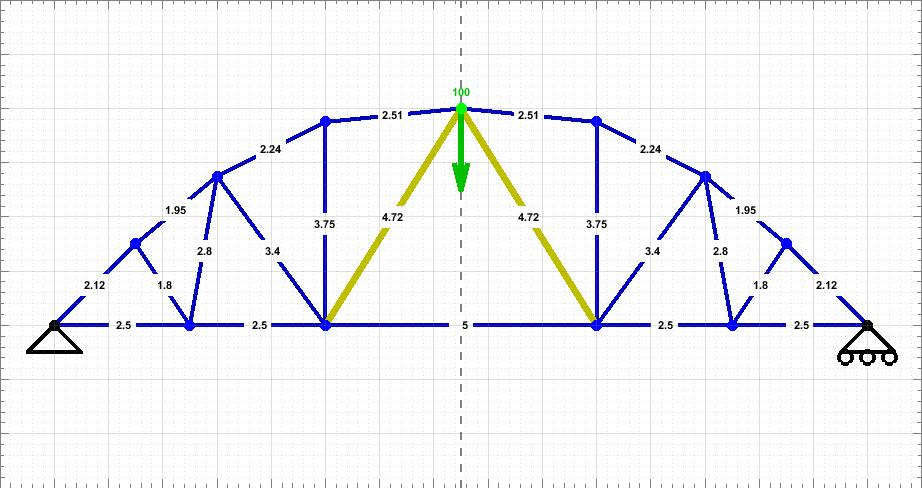
\includegraphics[width=0.75\textwidth]{assets/final_truss_2_lengths.jpg}
  \label{fig:truss-lengths-alt-1}
  \caption{Alternative 1 Design Lengths}
\end{figure}

\newpage

Data

\bigskip

\centering
\csvautotabular{assets/final_truss_2.csv}

\newpage

\subsubsection{Alternative 2}

Forces

\begin{figure}[!htb]
  \centering
  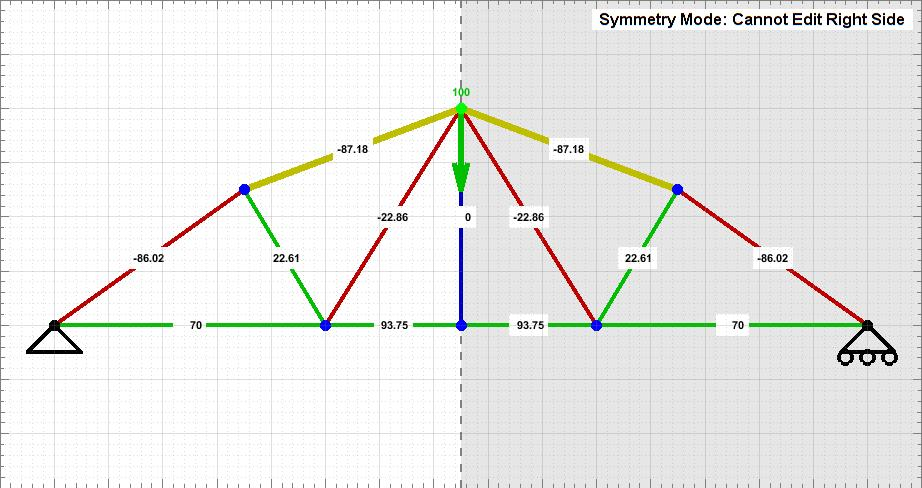
\includegraphics[width=0.75\textwidth]{assets/final_truss_3_forces.jpg}
  \label{fig:truss-forces-alt-2}
  \caption{Alternative 2 Design Forces}
\end{figure}

Lengths

\begin{figure}[!htb]
  \centering
  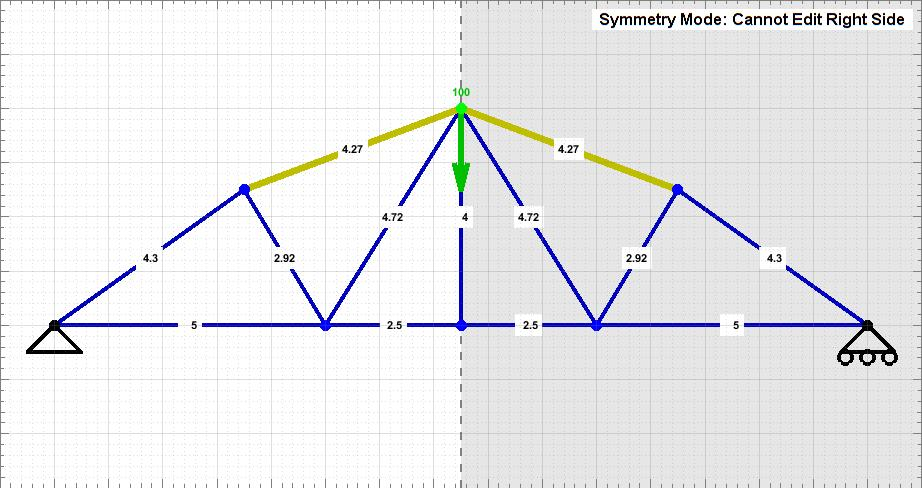
\includegraphics[width=0.75\textwidth]{assets/final_truss_3_lengths.jpg}
  \label{fig:truss-lengths-alt-2}
  \caption{Alternative 2 Design Lengths}
\end{figure}

\newpage

Data

\bigskip

\centering
\csvautotabular{assets/final_truss_3.csv}

\newpage

\begin{sidewaysfigure}

\subsection{Data}

\bigskip

\subsubsection{Results}

\bigskip

\begin{tabular}{lllllllll}
D3 SECTION S &  &  &  &  &  &  &  &  \\
Name & T & Design &  &  & Results &  &  &  \\
 &  & Load(lbs) & Length(in) & Load/Len Ratio & Weight(g) & Mass/Len Ratio & Load Failure(lbs) & Load Error(\%) \\
Albarella, Domenico & 1 & 424.7 & 67.43 & 6.3 & 93 & 1.38 & 448 & 5.5 \\
Cooper, Anna &  &  &  &  &  &  &  &  \\
Kennedy, Sean &  &  &  &  &  &  &  &  \\
Balgahoom, Jordan & 2 & 447 & 66.2 & 6.8 & 90 & 1.36 & 475 & 6.3 \\
Chesterman, Andrew &  &  &  &  &  &  &  &  \\
Schmidt, Joshua &  &  &  &  &  &  &  &  \\
Cimicata, Christopher & 3 & 375.2 & 58.93 & 6.4 & 85 & 1.44 & 120 & -68.0 \\
Daly, Hunter &  &  &  &  &  &  &  &  \\
Knurek, Sophia &  &  &  &  &  &  &  &  \\
Deitz, Joseph & 4 & 346.1 & 66.68 & 5.2 & 88 & 1.32 & 275 & -20.5 \\
Li, David &  &  &  &  &  &  &  &  \\
Pugliese, Jamie &  &  &  &  &  &  &  &  \\
Dupuy, Matthieu & 5 & 467.6 & 67.52 & 6.9 & 128 & 1.90 & 463 & -1.0 \\
Liu, Yijun &  &  &  &  &  &  &  &  \\
Sparta, Nicholas &  &  &  &  &  &  &  &  \\
Capron, Chase & 6 & 350 & 59.8 & 5.9 & 89 & 1.49 & 154 & -56.0 \\
Galas, Robert &  &  &  &  &  &  &  &  \\
Schwiebert, Joan &  &  &  &  &  &  &  &  \\
Maurelli, Mark & 7 & 506 & 68.34 & 7.4 & 107 & 1.57 & 436 & -13.8 \\
Sloat, James &  &  &  &  &  &  &  &  \\
Smith, Connor &  &  &  &  &  &  &  &  \\
Froehlich, Brynn & 8 & 346.1 & 68.9 & 5.0 & 106 & 1.54 & 398 & 15.0 \\
Thomson, Benjamin &  &  &  &  &  &  &  &  \\
Underwood, Andrew &  &  &  &  &  &  &  & 
\end{tabular}

\end{sidewaysfigure}

\newpage

\begin{sidewaysfigure}

\subsubsection{Individual Work}

\bigskip

\begin{tabular}{lllll}
Name & Action 1 & Action 2 & Action 3 & Action 4 \\
Jordan & Designed Truss & Sanded members, make them fit & Measured gusset plates & Soldered gusset plates onto joints \\
Josh & Created Truss & Cut members from brass tubing & Cut gusset plates & Soldered gusset plates to attach to joints \\
Andrew & Planned Truss & Sanded members & Sanded gusset plates & Attached gusset plates to joints using the solder
\end{tabular}

\end{sidewaysfigure}

%\printbibliography

\end{document}